\chapter{Architektur und Inbetriebhnahme von lokalen Apache Spark Infrastrukturen }
\label{chapter:architektur}



Im folgenden Kapitel wird ein exemplarischer Architekturaufbau eines lokalen Entwicklungs- und Testsystems für Apache Spark vorgestellt. Wie in den vorangegangen Kapiteln gezeigt wurde, handelt es sich bei Spark in erster Linie um ein Framework für leistungsstarke Clustersysteme. Dennoch muss Spark auch auf entsprechend kleiner dimensionierten System betrieben werden können. Häufig ist in einem professionellen Umfeld beispielsweise nur ein Cluster für Produktionsaufgaben vorhanden, die Test- und vor allem auch die Entwicklersysteme stellen sich häufig in Form sogenannter \textit{SIngle-Node-Cluster} dar. 

Besonders der Aspekt der Entwicklungsarbeitsplätze rückt hier in den Vordergrund. Da Spark lediglich über den \textit{Master-Node} und hier über den \textit{Spark-Context} innerhalb des \textit{Driver-Program} für die Entwickler zugreifbar ist und die interne Verteilung der Tasks auf die jeweiligen \textit{Nodes} von Spark und den \textit{Clustermanagement-Systemen} übernommen und maskiert wird, stellt sich die Fehleranalyse mittels klassischem \textit{Debugging}\footnote{Unter klassischem Debugging wird hier das Setzen von Breakpoints und das explizite Überwachen von Variablenwerten zur Laufzeit durch Entwickler verstanden.} als sehr große Herausforderung dar. Problematisch ist hierbei in erster Linie, dass vor und während des Debugging-Prozesses zu keiner Zeit der aktuelle Ausführungs-Node im Cluster determiniert werden kann. Da auf jedem \textit{Node} eine unabhängige \textit{JVM}\footnote{JVM = Java Virtual Machine. Hierbei handelt es sich um die Laufzeitumgebung von Java. Auch Scala-Code wird intern in Bytecode übersetzt und innerhalb der JVM ausgeführt.} instanziert ist, kann nicht zentral ermittelt und nachvollzogen werden, wo und zu welchem Ausführungszeitpunkt welches Verhalten auftritt. Für initiale Entwicklungstätigkeiten ist aus diesen Gründen immer eine lokale Instanz von Spark als Single-Node-Cluster nötig.

Zum Zweck von Versuchen bezüglich Skalierbarkeit im Cluster-Umfeld und Verhalten im verteilten Betrieb empfiehlt es sich, darüber hinaus eine lokale Cluster-Infrastruktur mit mindestens einem Master-und einem unabhängigen Worker-Node zu installieren. Dies kann auf verschiedene Arten stattfinden. Im Rahmen dieser Ausarbeitung wurden verschiedene Konfigurationen aufgebaut und miteinander verglichen. Diese Aufbauten mit ihren jeweiligen Stärken und Schwächen werden im folgenden Kapitel beschrieben. 

Des weiteren wird die Installation und die grundsätzliche Anwendung der Bibliotheken rund um Spark, bzw. der Alternativimplementierungen gezeigt. Abschließend werden Empfehlungen für verschiedene Einsatzbereiche gegeben. 

\section{Prinzipieller Aufbau einer lokalen Spark Infrastruktur}
\label{section:prinzipiell}

Eine Spark-Infrastruktur besteht immer aus verschiedenen Schichten, von denen einige zwingend notwendig sind, einige optional und andere durch Alternativimplementierungen ersetzt werden können.  
In Abbildung \ref{fig:bdas]} ist der Aufbau des BDAS schematisch dargestellt. Die grün hinterlegten Elemente markieren die Bestandteile des aktuellen BDAS, die violett hinterlegten zeigen alternative Implementierungen auf der jeweiligen Schicht. Grün schraffiert ist die Applikationsschicht, wo Applikationen oberhalb von Spark und den direkten Anwendungen angesiedelt sind. 

\begin{figure}[htb!]
\centering
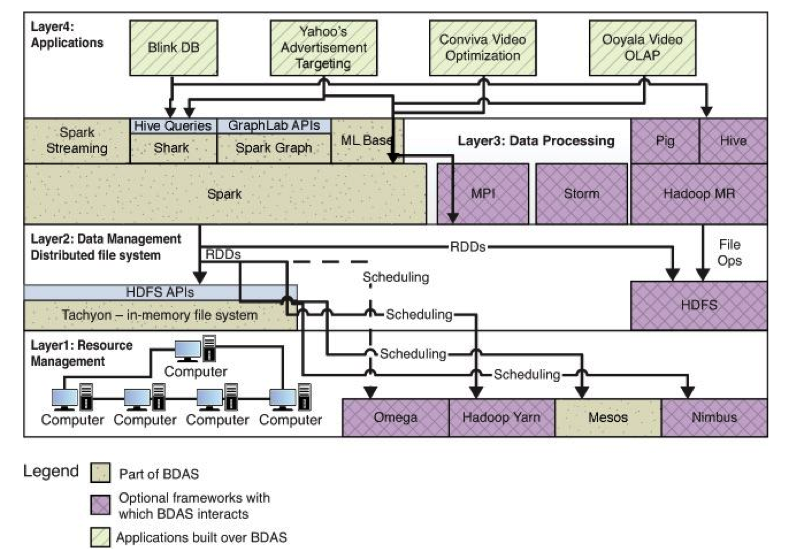
\includegraphics[width=1.0\textwidth]{bilder/2_2_stack.png}
\caption{Der BDAS. Abbildung aus „Big Data Analytics Beyond Hadoop“, S 15 \protect\citelit{va14}}
\label{fig:bdas]}
\end{figure} 

Der BDAS beginnt in der untersten Schicht mit Mesos oder einer seiner Alternativen. Für eine lokale Installation von Spark wird allerdings in der Regel keine eigenes Cluster-Resource-Management-System benötigt, da Spark die Grundfunktionalitäten für die Ressourcenverwaltung selbst im Kernel implementiert hat. 

Prinzipiell ist zunächst zu entscheiden, ob Spark lokal als Single- oder Mulitnode-Cluster betrieben werden soll. Diese Entscheidung sollte auch maßgeblich von der zur Verfügung stehenden Hardware abhängig gemacht werden und von den Einsatzgebieten. Sind die Tasks gut parallelisierbar, bietet sich ein Cluster aus Master und \(1...n\) Worker-Nodes an, ansonsten sollte den einzelnen Knoten oder einem Single-Node-Cluster möglichst viel Hauptspeicher zur Verfügung gestellt werden um die Festspeicherzugriffe zu minimieren. 

Da Spark durch seine beiden Hauptmerkmale \textit{In-Memory-Computation} und \textit{massive Parallelverarbeitung} eine möglichst starke Hardwareinfrastruktur benötigt und hier besonders die Aspekte Hauptspeicher, Prozessorkerne, Knotenanzahl und Netzwerkperformance essentiell sind, sollte generell ist eine lokale Spark-Installation so einfach wie möglich aufgebaut werden. Der Fokus sollte hier auf Entwicklungstätigkeit, Debugging, und Vergleichsmessungen gelegt werden. 

Für die lokale Installation besteht die Möglichkeit, Spark nativ auf dem System zu installieren, oder in virtualisierten Umgebungen. Eine native Installation hat den Vorteil, dass Spark eine systemnahe JVM als Ausführungsumgebung zum Einsatz kommt. So kann ein Großteil der vorhandenen Systemressourcen für die Spark-Ausführung zur Verfügung gestellt werden. Eine native Installation lässt sich entweder als Single-Node (Master-Only) konfigurieren, oder als virtuelles Cluster mit einem Master und einem Worker-Node. Hier empfiehlt sich ein Hybridbetrieb. Für Debugging-Aufgaben ist auf Grund der Taskverteilung von Spark nur ein Single-Node-Einsatz praktikabel. Für Skalierbarkeitstests bietet sich das Setup mit einem Master und einem Worker-Node an. 

Als Alternativen zu dieser nativen Installation lässt sich ein theoretisch beliebig großes virtuelles Cluster auf einer lokalen Umgebung mit einer entsprechenden Anzahl von virtuellen Maschinen realisieren. Dies hat den Vorteil, dass die Skalierbarkeit der Anwendung durch entsprechende Partitionierung der RDDs besser testbar ist. Allerdings haben virtuelle Maschinen in der Regel einen sehr hohen Ressourcenverbrauch und lassen so nur bedingt Rückschlüsse auf das tatsächliche Laufzeitverhalten zu. 

Eine weitere Möglichkeit des Setups ist das Deployment der kompletten Spark-Infrastruktur in einen Docker-Container. Diese Möglichkeit wird im folgenden Unterkapitel \ref{section:docker} beschrieben. 

\newpage 


\section{Ausführungscontainer: Docker}
\label{section:docker}

Bei Docker handelt es sich um eine Open-Source-Plattform zur Automatisierung des Software-Deployments innerhalb von Ausführungscontainern \citeint{do15}. Prinzipiell legt Docker eine weitere Abstraktionsschicht über ein vorhandenes Linux-System und nutzt dessen \textit{Resource-Isolation-Features}, wie beispielsweise \textit{cgroups}\footnote{Bei cgroups handelt es sich um eines der Linux-Kernel-Features, um Ressourcen (CPU, Speicher, I/O, etc.) für verschiedene Prozesse isolieren zu können. Weitere RIFs sind \textit{capabilities, namespaces, SELinux, Netlink, Netfilte, AppAmor} (Vergleich \citelit{cbo14})} \citeint{dol14}. 

Durch Docker werden isolierte Prozesse mittels \textit{High-Level-API} in leichtgewichtigen Ausführungscontainern erzeugt. Der Vorteil gegenüber herkömmlichen Virtualisierungstechnologien, wie beispielsweise Oracle Virtual Box, Citrix XenServer, VMWare, besteht unter anderem darin, dass bei Docker im Gegensatz zu diesen Applikationen kein eigenes Betriebsystem in einer virtuellen Maschine installiert werden muss. Dadurch sind Docker-Container äußerst ressourcenschonend. Voraussetzung für einen Betrieb von Docker ist allerdings ein installiertes Linux-Betriebssystem auf dem Hostrechner. Docker bietet die Möglichkeit, relativ kleine Services in eigenen Containern unterzubringen. Die Prinzipien einer \textit{Microservice-Infrastruktuktur}\footnote{Microservices sind ein Designpattern in der Softwarearchitektur, in dem komplexe Anwendungen in kleine, unabhängige Services ausgelagert werden. Diese können mittels verschiedener Sprachen entwickelt werden und stellen ihre jeweilige API den Konsumenten zur Verfügung.}, allen voran die \textit{Immutability}\footnote{Unter Immutability versteht man in der objektorientierten und funktionalen Programmierung, dass ein Objekt nach dessen Erzeugung nicht mehr modifiziert werden kann.}, können so mittels Docker-Containern umgesetzt werden  (Vergleich \citeint{do15}). 

Docker ist sehr gut geeignet, eine lokale Apache Spark Infrastruktur aufzusetzen und diese inklusive aller Abhängigkeiten und deployten Anwendungen sowohl an andere Standalone-, als auch an Clustersysteme auf sehr einfache Weise zu verteilen. Bei der lokalen Installation mit Docker-Containern besteht die Wahl zwischen einer portablen Single-Node-Umgebung und einem virtualisierten Cluster. Prinzipiell gelten für den Fall der Docker-Installation die gleichen Bedingungen, wie für eine native Installation. Darüber hinaus lässt ein Setup mit Docker-Containern auch mehr als einen Worker-Node zu. Doch auch hier muss beachtet werden, dass Spark seine Stärken beim In-Memory-Processing nur mit ausreichenden Ressourcen nutzen kann. Auch wenn Docker eine sehr leichtgewichtige Virtualisierungslösung darstellt, muss dennoch beachtet werden, dass hier nicht die vollen Ressourcen wie bei einer nativen Installation zur Verfügung stehen. 

Bereits konfigurierte Docker-Container können in einer eigenen Plattform, dem sogenannten Docker Hub verwaltet, mit anderen Nutzern geteilt und heruntergeladen werden. 

Im Folgenden wird exemplarisch gezeigt, wie ein Docker Container für Apache Spark aufgebaut, konfiguriert und deployt werden kann \citeint{ms15}. Dieser Container wurde auf einem Windows Hostrechner innerhalb einer VirtualBox-Instanz erstellt. Diese virtuelle Maschine wurde mit einer leichtgewichtigen CentOS-Installation aufgebaut. 

Da CentOS auf einer RedHat-Linuxdistribution aufsetzt, wird als Paketmanager \textit{YUM} eingesetzt. Für die einfache Provisionierung der Docker Container bietet sich Vagrant ab Version 1.6 an \citeint{vag14}. So lassen sich die Docker Container mittels entsprechender Scripts einfach konfigurieren. 

\begin{lstlisting}[label=vagrant setup jvm-spark,caption=Setup JVM with Spark]
FROM jvm
RUN yum clean all
RUN yum install -y tar yum-utils wget
RUN yum-config-manager --save 
RUN yum update -y
RUN yum install -y java-1.8.0-openjdk-devel.x86_64
COPY spark-1.2.0-bin-hadoop2.4.tgz /opt/
RUN tar -xzf /opt/spark-1.2.0-bin-hadoop2.4.tgz -C /opt/
RUN echo "SPARK_HOME=/opt/spark-1.2.0-bin-hadoop2.4" >> /etc/environment
RUN echo "JAVA_HOME=/usr/lib/jvm/java-1.8.0-openjdk/" >> /opt/spark-1.2.0-bin-hadoop2.4/conf/spark-env.sh

\end{lstlisting}

\begin{lstlisting}[label=vagrant setup jvm-spark,caption=Setup JVM with Spark]
# number of instances : First one is master.
$spark_num_instances = 2
$cassandra_num_instances = 1
Vagrant.configure("2") do |config|
    # nodes definition
    (1..$spark_num_instances).each do |i|
        config.vm.define "scale#{i}" do |scale|
            scale.vm.provider "docker" do |d|
                d.build_dir = "spark/"
                d.name = "scale#{i}"
                d.create_args = ["--privileged=true"]
                d.remains_running = true
                if "#{i}" == "1"
                    d.ports = [ "4040:4040", "7707:7707" ] 
                else
                    d.create_args = d.create_args << "--link" << "scale1:scale1.docker"
                end
            end
            scale.vm.synced_folder "./", "/scale-shared/"
            scale.vm.hostname = "scale#{i}.docker"
       end 
    end

\end{lstlisting}




  

\section{Cluster Management: Mesos und Yarn }
\label{section:mesos}

Blablba

\section{Caching-Framework: Tachyon}
\label{section:tachyon}

Blablba

\section{Der eigentliche Kern: Apache Spark}
\label{section:kern}

Blablba

\section{Streaming-Framework: Spark Streaming}
\label{section:streaming}

Blablba

\section{Abfrageschicht: Spark SQL}
\label{section:spark sql}

Blablba

\section{Machine Learning Algorithmen: MLLib}
\label{section:mllib arch}

Blablba



\section{Graphenanwendungen: GraphX}
\label{section:graphx}

Blablba

\section{Einrichten und Konfigurieren der IDE IntelliJ Idea für Spark}
\label{section:intellij}

Blablba

\section{Alternativimplementierung zu MLLibs: H2O}
\label{section:h2o}

Blablba

\section{Alternativimplementierung zu Spark: Apache Flink}
\label{section:h2o}

Blablba

